% This is "sig-alternate.tex" V2.1 April 2013
% This file should be compiled with V2.5 of "sig-alternate.cls" May 2012
%
% This example file demonstrates the use of the 'sig-alternate.cls'
% V2.5 LaTeX2e document class file. It is for those submitting
% articles to ACM Conference Proceedings WHO DO NOT WISH TO
% STRICTLY ADHERE TO THE SIGS (PUBS-BOARD-ENDORSED) STYLE.
% The 'sig-alternate.cls' file will produce a similar-looking,
% albeit, 'tighter' paper resulting in, invariably, fewer pages.
%
% ----------------------------------------------------------------------------------------------------------------
% This .tex file (and associated .cls V2.5) produces:
%       1) The Permission Statement
%       2) The Conference (location) Info information
%       3) The Copyright Line with ACM data
%       4) NO page numbers
%
% as against the acm_proc_article-sp.cls file which
% DOES NOT produce 1) thru' 3) above.
%
% Using 'sig-alternate.cls' you have control, however, from within
% the source .tex file, over both the CopyrightYear
% (defaulted to 200X) and the ACM Copyright Data
% (defaulted to X-XXXXX-XX-X/XX/XX).
% e.g.
% \CopyrightYear{2007} will cause 2007 to appear in the copyright line.
% \crdata{0-12345-67-8/90/12} will cause 0-12345-67-8/90/12 to appear in the copyright line.
%
% ---------------------------------------------------------------------------------------------------------------
% This .tex source is an example which *does* use
% the .bib file (from which the .bbl file % is produced).
% REMEMBER HOWEVER: After having produced the .bbl file,
% and prior to final submission, you *NEED* to 'insert'
% your .bbl file into your source .tex file so as to provide
% ONE 'self-contained' source file.
%
% ================= IF YOU HAVE QUESTIONS =======================
% Questions regarding the SIGS styles, SIGS policies and
% procedures, Conferences etc. should be sent to
% Adrienne Griscti (griscti@acm.org)
%
% Technical questions _only_ to
% Gerald Murray (murray@hq.acm.org)
% ===============================================================
%
% For tracking purposes - this is V2.0 - May 2012

\documentclass{sig-alternate-05-2015}

% *** CITATION PACKAGES ***
\usepackage{cite}

% *** MATH PACKAGES ***
\usepackage{amsmath}
\usepackage{svg}
\usepackage{amsfonts}

% *** PDF, URL AND HYPERLINK PACKAGES ***
\usepackage{url}
\usepackage{hyperref}
\usepackage{epigraph}

% *** ALGORITHM ***
%\usepackage{algorithm}
%\usepackage{algpseudocode}
\usepackage[ruled, linesnumbered]{algorithm2e}
\renewcommand{\algorithmcfname}{ALGORITHM}
\SetAlFnt{\small}
\SetAlCapFnt{\small}
\SetAlCapNameFnt{\small}
\SetAlCapHSkip{0pt}
\IncMargin{-\parindent}

\usepackage{booktabs}
\usepackage{enumitem}

% *** To balance reference page ***
\usepackage{flushend}

% *** Draw diagrams ***
\usepackage{tikz}
\usetikzlibrary{positioning}
\usetikzlibrary{arrows.meta}

% *** Fancy Table ***
\usepackage{multirow}

\newcommand{\paragraphb}[1]{\vspace{0.03in}\noindent{\bf #1} }
\newcommand{\paragraphe}[1]{\vspace{0.03in}\noindent{\em #1} }
\newcommand{\paragraphbe}[1]{\vspace{0.03in}\noindent{\bf \em #1} }

\newcommand{\kevin}[1]{{\color{red}{#1}}} 
\newcommand{\kevinc}[1]{{\color{red}\bf\em{[kevin: #1]}}} 

\newcommand{\name}{DSSnet\xspace}
\newcommand{\Name}{DSSnet\xspace}

\newtheorem{lemma}{Lemma}
\newtheorem{theorem}{Theorem}
\newdef{definition}{Definition}

% *** For commenting blocks of text ***
%\newcommand{\CUT}[1]{{}}
\begin{document}

%\begin{comment}
% DOI
%\doi{000-0-0000-0 00-0}

% ISBN
%\isbn{0000000/0000}

\CopyrightYear{2017} \setcopyright{acmcopyright}
\conferenceinfo{SIGSIM-PADS '17,}{May 24--26, 2017, Singapore.}
\isbn{xxx-x-xxxx-xxxx-x/xx/xx}\acmPrice{\$15.00}
\doi{http://dx.doi.org/xx.xxxx/xxxxxxxxxx.xxxxxx}
%Authors, replace the red X's with your assigned DOI string.
\clubpenalty=10000
\widowpenalty = 10000
%\end{comment}
 
%
% --- Author Metadata here ---
%\conferenceinfo{WOODSTOCK}{'97 El Paso, Texas USA}
%\CopyrightYear{2007} % Allows default copyright year (20XX) to be over-ridden - IF NEED BE.
%\crdata{0-12345-67-8/90/01}  % Allows default copyright data (0-89791-88-6/97/05) to be over-ridden - IF NEED BE.
% --- End of Author Metadata ---

\title{Simulating Entire SDN Network as An OpenFlow Switch}
%\subtitle{[BigSimSwitch]
%\titlenote{code for our project available on www.github.com}}

%
% You need the command \numberofauthors to handle the 'placement
% and alignment' of the authors beneath the title.
%
% For aesthetic reasons, we recommend 'three authors at a time'
% i.e. three 'name/affiliation blocks' be placed beneath the title.
%
% NOTE: You are NOT restricted in how many 'rows' of
% "name/affiliations" may appear. We just ask that you restrict
% the number of 'columns' to three.
%
% Because of the available 'opening page real-estate'
% we ask you to refrain from putting more than six authors
% (two rows with three columns) beneath the article title.
% More than six makes the first-page appear very cluttered indeed.
%
% Use the \alignauthor commands to handle the names
% and affiliations for an 'aesthetic maximum' of six authors.
% Add names, affiliations, addresses for
% the seventh etc. author(s) as the argument for the
% \additionalauthors command.
% These 'additional authors' will be output/set for you
% without further effort on your part as the last section in
% the body of your article BEFORE References or any Appendices.


%\begin{comment}
\numberofauthors{3} %  in this sample file, there are a *total*
% of EIGHT authors. SIX appear on the 'first-page' (for formatting
% reasons) and the remaining two appear in the \additionalauthors section.
%

\author{
% You can go ahead and credit any number of authors here,
% e.g. one 'row of three' or two rows (consisting of one row of three
% and a second row of one, two or three).
%
% The command \alignauthor (no curly braces needed) should
% precede each author name, affiliation/snail-mail address and
% e-mail address. Additionally, tag each line of
% affiliation/address with \affaddr, and tag the
% e-mail address with \email.
%
% 1st. author
\alignauthor
Jiaqi Yan\\
      \affaddr{Illinois Institute of Technology}\\
       \affaddr{10 West 31st Street}\\
       \affaddr{Chicago, Illinois, 60616 }\\
       \email{jyan31@hawk.iit.edu}
% 2nd. author
\alignauthor
Xin Liu\\
       \affaddr{Illinois Institute of Technology}\\
       \affaddr{10 West 31st Street}\\
       \affaddr{Chicago, Illinois, 60616 }\\
       \email{xliu125@hawk.iit.edu}
% 3rd. author
\alignauthor
Dong Jin\\
       \affaddr{Illinois Institute of Technology}\\
       \affaddr{10 West 31st Street}\\
       \affaddr{Chicago, Illinois, 60616 }\\
       \email{dong.jin@iit.edu}
%\and  % use '\and' if you need 'another row' of author names
%% 4th. author
%\alignauthor Lawrence P. Leipuner\\
%       \affaddr{Brookhaven Laboratories}\\
%       \affaddr{Brookhaven National Lab}\\
%       \affaddr{P.O. Box 5000}\\
%       \email{lleipuner@researchlabs.org}
%% 5th. author
%\alignauthor Sean Fogarty\\
%       \affaddr{NASA Ames Research Center}\\
%       \affaddr{Moffett Field}\\
%       \affaddr{California 94035}\\
%       \email{fogartys@amesres.org}
%% 6th. author
%\alignauthor Charles Palmer\\
%       \affaddr{Palmer Research Laboratories}\\
%       \affaddr{8600 Datapoint Drive}\\
%       \affaddr{San Antonio, Texas 78229}\\
%       \email{cpalmer@prl.com}
}

%\end{comment}

\maketitle
\begin{abstract}
To do
\end{abstract}


%
% The code below should be generated by the tool at
% http://dl.acm.org/ccs.cfm
% Please copy and paste the code instead of the example below. 
%
\begin{comment}
\begin{CCSXML}
<ccs2012>
 <concept>
  <concept_id>10010520.10010553.10010562</concept_id>
  <concept_desc>Computer systems organization~Embedded systems</concept_desc>
  <concept_significance>500</concept_significance>
 </concept>
 <concept>
  <concept_id>10010520.10010575.10010755</concept_id>
  <concept_desc>Computer systems organization~Redundancy</concept_desc>
  <concept_significance>300</concept_significance>
 </concept>
 <concept>
  <concept_id>10010520.10010553.10010554</concept_id>
  <concept_desc>Computer systems organization~Robotics</concept_desc>
  <concept_significance>100</concept_significance>
 </concept>
 <concept>
  <concept_id>10003033.10003083.10003095</concept_id>
  <concept_desc>Networks~Network reliability</concept_desc>
  <concept_significance>100</concept_significance>
 </concept>
</ccs2012>  
\end{CCSXML}

\ccsdesc[500]{Computer systems organization~Embedded systems}
\ccsdesc[300]{Computer systems organization~Redundancy}
\ccsdesc{Computer systems organization~Robotics}
\ccsdesc[100]{Networks~Network reliability}

%
% End generated code
%
\end{comment}
%
%  Use this command to print the description
%
%\printccsdesc

% We no longer use \terms command
%\terms{Theory}

\keywords{Network Emulation; Software-Defined Networking;}

\section{Introduction}

% Bring in the issues that our approach can address
% Describe them as problems in current simulation/emulation systems
Software defined networking (SDN) explicitly separate the logic of the network
from the distributed hardware that implementing the forwarding behaviors.
This centralized scheme have been widely adopted in datacenters networks
and internet exchange points\cite{B4, Meridian, SDX}.
However, similar to traditional computer network systems, it is still crucial to do testing
and evaluating before deployment.
Consequently researchers in the simulation community have extend various
traditional network simulators to provide SDN support\cite{S3F, NS3, OPNET}.
Though network simulation is both reproducible and scalable,
people are not always confident with its fidelity due to its idealized modelling process.
In contrast, researcher in SDN community propose container-based emulation that utilize
shared hardware resources and real network stack to run high-fidelity SDN experiments\cite{Mininet}.
However, the experiment scale is limited to the resources available on the running machine.
For example in a traditional tree-topology network with depth 4 and fanout 10,
we need to start up 1111 switches and 10000 hosts.
If we want to achieve full connectivity, we need to install at least 799,920,000(=8 * 10000 * 9999)
OpenFlow rules in total.
Assuming rules only have source IP address, destination IP address, inport number and outport number,
each rule will consume at least 10 Bytes memory, meaning around 7.45 GB of memory are required to
emulate this network.
Such intensive resource requirement are not commonly satisfied by commodity low-end machines.

% State our idea
In this work we propose to address the scalability issue by simplifying the emulated
SDN network both logically and physically.
Inspired by works of~\cite{OneBigSwitchAbstraction, Veriflow},
we abstract a subset of the networked SDN switches as \textbf{one} big switch.
In the very extreme case, the entire set of the SDN switches are compressed to
one OpenFlow switch.
The obvious benefit is the much less number of switches and/or number of rules existing in the network.
For the example mention above, we only need to start up one switch and 10000 hosts.
On the single switch, we only need to install about 99,990,000 rules, requiring about 1 GB memory.
Besides, the abstracted big switch can be used in multiple plug-in-play scenarios.
For example, researchers can reproduce the simulation result with very
simple configurations (link connectivity setup, flow table configuration etc.)
after one complex run on the original network.
In the case of a too-large-to-simulate network, we can divide it into subsets of switches,
abstract each subset separately.
Then we are able to combine multiple big switches together and emulating the size-reduced network.

The big switch must preserve \textbf{packet-level fidelity} so that
it can be used with confidence in simulation or emulation.
More concretely, we need to abstract the SDN network under two constraints:
\begin{itemize}
\item \textbf{Logic Equivalence.} The forwarding behavior of any packet must be identical
        between both representations of the real network. Packets being
        forwarded through out the network (1) will also be forwarded through out
        some interface of the big switch, (2) any modifications made by
        intermediate switches must be made by the big switch in proper order.
        Packets being dropped at some point in the network path will be drop by the
        big switch.
\item \textbf{Performance Equivalence.} A packet transmitted through a series of
        switches can be seen as processed by multiple queueing systems $\mathcal{Q}$.
        Similarly, the packet processing performance model in a big OpenFlow switch can
        also be modeled as a queueing system $Q$.
        The parameters of the later should be configured so that per packet performance
        measurements are as closed as possible to the ones in the former composite model.
        As an informal example, queueing delay for packet $p$, $Q(p, T)$, should be an
        function that approximates $\mathcal{Q}(p, T')$.
\end{itemize}

While our long term goal is to propose systematic approaches and algorithms to reduce
networked SDN switches to one switch that satisfies both logical equivalence and performance
equivalence, in this work, we mainly focus on the former constraint.
To preserve the forwarding logic in a group of interconnected OpenFlow switches,
we first classify all the possible packets (equivalence classes) by iterating through
the match fields in each rules in the network;
then we model each class of packet's forwarding behavior by create forwarding graphs;
at last one rule will be generated at the end of forwarding graph traversal.
This three-step process is illustrated in Figure~\ref{Fig:BigSimOverview} and discussed
in detail in Section~\ref{Sec:Design}.
Our contributions include:
\begin{itemize}
\item We apply the reversed idea of ``One Big Switch"\cite{OneBigSwitchAbstraction}
        to SDN network simulation or emulation in order to
        improve their scalability and reusability.
\item Built on the idea of equivalence class and forwarding graph, we design
        a systematic approach to compress all the rules in a SDN network without
        loss of forwarding logic.
\item For several phases in our approach, we propose corresponding optimization
        algorithms to reduce the time complexity.
\end{itemize}

\begin{figure}[t]
\centering
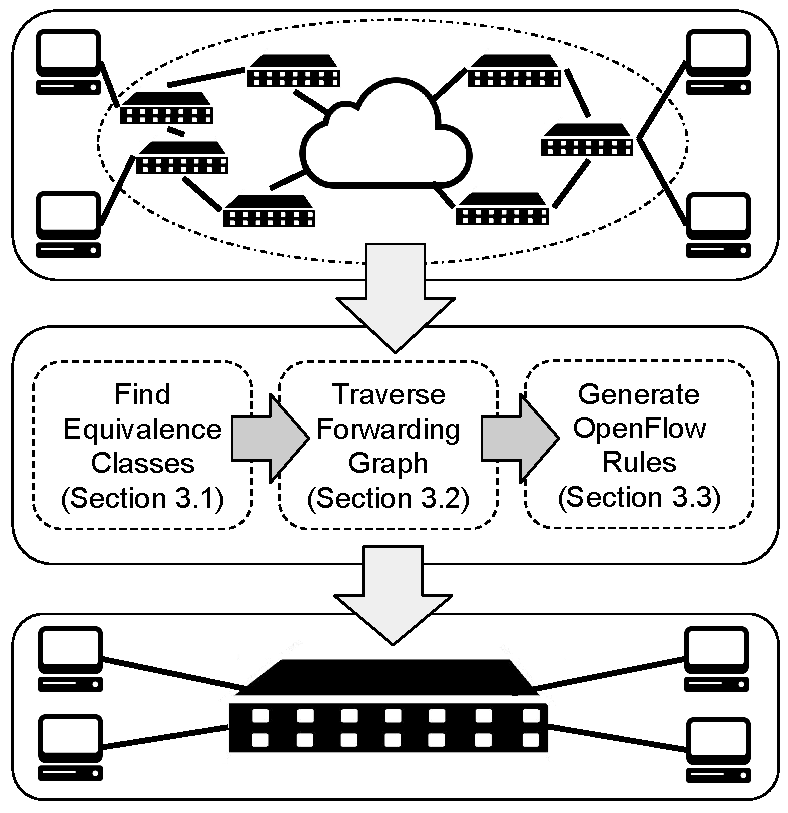
\includegraphics[scale=.6]{figures/BigSimOverview.pdf}
\caption{BigSim transforms a SDN network (controller is not shown for simplicity) to a virtual OpenFlow switch without the loss of forwarding logic.}
\label{Fig:BigSimOverview}
\end{figure}


\section{Motivational Example}
\label{Sec:MotivationalExample}

\tikzset {
        roundnode/.style={circle, draw=blue!80, fill=blue!5, very thick, minimum size=7mm},
        squarenode/.style={rectangle, draw=red!80, fill=red!5, very thick, minimum size=7mm},
        ->-/.style={->, line width=1.2pt},
        ==/.style={line width=1.6pt}
}

\begin{figure}[t]
\centering
\begin{tikzpicture}
\node[roundnode] (sw0) {SW0};
\node[roundnode] (sw1) [below left=2cm of sw0] {SW1};
\node[roundnode] (sw2) [below=1.1cm of sw0] {SW2};
\node[roundnode] (sw3) [below right=2cm of sw0] {SW3};
\node[squarenode] (net1) [below=1cm of sw1] {10.1.0.10/16};
\node[squarenode] (net2) [below=1cm of sw2] {10.0.0.10/8};
\node[squarenode] (net3) [below=1cm of sw3] {11.1.0.10/16};

\draw[-, line width=1.2pt] (sw0) -- node [near start, above] {0} node[near end, below] {1} (sw1);
\draw[-, line width=1.2pt] (sw0) -- node [near start, right] {1} node[near end, left] {1} (sw2);
\draw[-, line width=1.2pt] (sw0) -- node [near start, above] {2} node[near end, below] {1} (sw3);
\draw[-, line width=1.2pt] (sw1) -- node [near start, left] {0} (net1);
\draw[-, line width=1.2pt] (sw2) -- node [near start, left] {0} (net2);
\draw[-, line width=1.2pt] (sw3) -- node [near start, right] {0} (net3);
\end{tikzpicture}
\caption{A Tree-Topology SDN Network}
\label{Fig:ExampleNetworkTopo}
\end{figure}

\begin{figure*}
\centering
\subfloat[Forwarding Graph for EC1 and EC3] {
\begin{tikzpicture}
\node[roundnode] (sw2) {SW2};
\node[roundnode] (sw0) [left=of sw2] {SW0};
\node[roundnode] (sw1) [above left=of sw0] {SW1};
\node[roundnode] (sw3) [below left=of sw0] {SW3};
\node[squarenode, align=center] (ec13) [right=of sw2] {EC1: 10.0.*.*\\EC3: 10.2.0.0-10.255.255.255};

\draw[->-] (sw0) -- node [near start, above] {1} node[near end, above] {1} (sw2);
\draw[->-] (sw1) -- node [near start, above] {1} node[near end, above] {0} (sw0);
\draw[->-] (sw3) -- node [near start, above] {1} node[near end, above] {2} (sw0);
\draw[->-] (sw2) -- node [near start, above] {0} (ec13);
\end{tikzpicture}
\label{Fig:ExampleForwardingEC13}
}

\subfloat[Forwarding Graph for EC2] {
\begin{tikzpicture}
\node[roundnode] (sw1) {SW1};
\node[roundnode] (sw0) [left=of sw2] {SW0};
\node[roundnode] (sw2) [above left=of sw0] {SW2};
\node[roundnode] (sw3) [below left=of sw0] {SW3};
\node[squarenode] (ec2) [right=of sw1] {EC2: 10.1.*.*};

\draw[->-] (sw0) -- node [near start, above] {0} node[near end, above] {1} (sw1);
\draw[->-] (sw2) -- node [near start, above] {1} node[near end, above] {1} (sw0);
\draw[->-] (sw3) -- node [near start, above] {1} node[near end, above] {2} (sw0);
\draw[->-] (sw1) -- node [near start, above] {0} (ec2);
\end{tikzpicture}
\label{Fig:ExampleForwardingEC2}
}
\subfloat[Forwarding Graph for EC4] {
\begin{tikzpicture}
\node[roundnode] (sw3) {SW3};
\node[roundnode] (sw0) [left=of sw3] {SW0};
\node[roundnode] (sw1) [above left=of sw0] {SW1};
\node[roundnode] (sw2) [below left=of sw0] {SW2};
\node[squarenode] (ec4) [right=of sw3] {EC4: 11.1.*.*};

\draw[->-] (sw0) -- node [near start, above] {2} node[near end, above] {2} (sw3);
\draw[->-] (sw1) -- node [near start, above] {1} node[near end, above] {0} (sw0);
\draw[->-] (sw2) -- node [near start, above] {1} node[near end, above] {1} (sw0);
\draw[->-] (sw3) -- node [near start, above] {0} (ec4);
\end{tikzpicture}
\label{Fig:ExampleForwardingEC4}
}
\caption{Forward Graph for Each EC}
\label{Fig:ExampleForwardingGraphs}
\end{figure*}

\begin{table*}[t]
\caption{Forwarding rules on each OpenFlow switch in the 3-ary tree topology network}
\begin{center}
\begin{tabular}{c|clc}
\hline
Switch & Priority & Match Field & Action\\
\hline
\hline
\multirow{3}{2em}{SW0} & 10 & NW\_DST=10.1.*.* & FWD: OUT\_PORT=0 \\
                       & 1  & NW\_DST=10.*.*.* & FWD: OUT\_PORT=1 \\
                       & 1  & NW\_DST=11.1.*.* & FWD: OUT\_PORT=2 \\
\hline
\multirow{3}{2em}{SW1} & 10 & IN\_PORT=1, NW\_DST=10.1.*.* & FWD: OUT\_PORT=0 \\
                       & 1  & IN\_PORT=0, NW\_DST=10.*.*.* & FWD: OUT\_PORT=1 \\
                       & 1  & IN\_PORT=0, NW\_DST=11.1.*.* & FWD: OUT\_PORT=1 \\
\hline
\multirow{3}{2em}{SW2} & 10 & IN\_PORT=0, NW\_DST=10.1.*.* & FWD: OUT\_PORT=1 \\
                       & 1  & IN\_PORT=1, NW\_DST=10.*.*.* & FWD: OUT\_PORT=0 \\
                       & 1  & IN\_PORT=0, NW\_DST=11.1.*.* & FWD: OUT\_PORT=1 \\
\hline
\multirow{3}{2em}{SW3} & 10 & IN\_PORT=1, NW\_DST=11.1.*.* & FWD: OUT\_PORT=0 \\
                       & 1  & IN\_PORT=0, NW\_DST=10.*.*.* & FWD: OUT\_PORT=1 \\
                       & 1  & IN\_PORT=0, NW\_DST=10.1.*.* & FWD: OUT\_PORT=1 \\
\hline
\end{tabular}
\end{center}
\label{Tab:OriginalFlowTable}
\end{table*}

\begin{table*}[t]
\caption{Forwarding Rules on the ``Big OpenFlow Switch"}
\begin{center}
\begin{tabular}{c|clc}
\hline
Switch & Priority & Match Field & Action\\
\hline
\hline
\multirow{4}{2em}{SW}  & 10 & NW\_DST=10.0.*.* & FWD OUT\_PORT=1 \\
                       & 10 & NW\_DST=10.1.*.* & FWD OUT\_PORT=0 \\
                       & 10 & NW\_DST=11.1.*.* & FWD OUT\_PORT=2 \\
                       & 10 & NW\_DST=10.2.0.0-10.255.255.255 & FWD OUT\_PORT=1 \\
\hline
\end{tabular}
\end{center}
\label{Tab:CompressedFlowTable}
\end{table*}

In this section, we describe our idea in a concrete network example and
walk through our method of how to compressing a SDN network to a ``big switch" module.
Let's consider the tree-topology network connected by 4 OpenFlow switches,
as shown in Figure~\ref{Fig:ExampleNetworkTopo}.
Centralized SDN controller(not shown in the figure) installs the rules shown in
Table~\ref{Tab:OriginalFlowTable} to each switch so that connection is established
for three subnets.
We assume the network has been in a stationary state, e.g. rules are already available
on each OpenFlow switch and there is no dynamic events occur such as link down
or rule modification.
SW0 then works properly as an \textbf{aggregate switch} to route traffic
between different subnets.
SW1, SW2 and SW3 play as \textbf{edge switches}, switches at the leave of the topology,
for three subnets respectively.
In this very special case, there is only one host connected to each edge switch.

Our approach abstracts the network composed of both aggregate switch and edge switches
to one ``big switch" that has logically equivalent functions.
The first step in the abstraction process is to extract \textit{equivalence classes}
through the OpenFlow rules from any devices in the network.
As formally defined later in Section~\ref{Sec:Design} and in \cite{Veriflow}, equivalence class (EC) is
the set of packets that experience identical forwarding action at \textbf{any} network device.
This concept is proposed to confine network verification activities to the minimal
effected set of packets\cite{Veriflow}.
In our approach, we utilize EC to merge all the rules on a set of switches.
For example, the flow rules shown in Table~\ref{Tab:OriginalFlowTable} can be sliced into
4 \textbf{disjoint} ECs based on the NW\_DST match field:
\begin{itemize}
\item Packets in EC1 is destined to network address 10.0.*.*.
\item Packets in EC2 is going to hosts with address 10.1.*.*.
\item Packets going to the address range from 10.2.0.0 to 10.255.255.255 belongs to EC3
\item Packets in EC4 goes to subnet 11.1.*.*. 
\end{itemize}
One thing to notice is that match field IN\_PORT cannot be used in identifying ECs,
since it is not packet-dependent but topology-dependent filed.

After identifying all the equivalence classes from the rule set,
we generate \textit{forwarding graph} which models how packets within an EC will be
forwarded through the network\cite{Veriflow}.
The node in a forwarding graph represents EC at a network device;
the directed edge represents how the network device forward the EC.
The sink nodes (shown as red rectangle node) is not part of the forwarding graph
but are drawn for recognizing which EC this forwarding graph belongs to.
If we skip the process of minimizing number of ECs from the rules,
each equivalence class will have exactly one forwarding graph.
Forwarding graph for all four ECs are shown separately in
Figure~\ref{Fig:ExampleForwardingGraphs}.
Notice that \{EC1, EC2, EC3, EC4\} is not the minimal set of ECs in the network.
In fact, EC1 and EC3 can be merged together because packets in both classes are forwarded
identically at any network device.
This is shown in Figure~\ref{Fig:ExampleForwardingEC13} as EC1 and EC3 share the same
forwarding graph.

We finish the abstraction by generating a new set of forwarding rules that are to be
installed on the ``big switch".
This process can be efficiently by considering only these ECs that
traverses edge switches in the abstracted network.
Table~\ref{Tab:CompressedFlowTable} shows the resulting rules that will be installed in
SW in Figure~\ref{Fig:ExampleBigSwitch}.

\begin{figure}[t]
\centering
\begin{tikzpicture}
\node[roundnode, minimum size=15mm, align=center] (sw) {Big\\Switch};
\node[squarenode, align=center] (ec13) [below=1.3cm of sw] {10.0.0.10/8};
\node[squarenode] (ec2) [below left=2cm of sw] {10.1.0.10/16};
\node[squarenode] (ec4) [below right=2cm of sw] {11.1.0.10/16};

\draw[-, line width=1.2pt] (sw) -- node [near start, above] {0} (ec2);
\draw[-, line width=1.2pt] (sw) -- node [near start, right] {1} (ec13);
\draw[-, line width=1.2pt] (sw) -- node [near start, above] {2} (ec4);
\end{tikzpicture}
\caption{Compressed SDN Network for Scalable Simulation}
\label{Fig:ExampleBigSwitch}
\end{figure}

The resulting one-switch network functions identical to the tree-topology network,
in the eyes of the three hosts(possibly emulated or simulated).
In contrast, the number of switches we need to emulate is reduced from four to one;
more importantly, the number of rules in the network is reduced from twelve to four.
If we confine the rules to these that (1) only match NW\_DST field;
(2) only have forwarding actions,
the total number of rules will be proportional to the number of ECs in the
original SDN network, comparing to $O(S\times P)$ where $S$ is the number of switches
and $P$ is the number of address prefixes.



\section{Design of BigSim}

\begin{figure}[t]
\centering
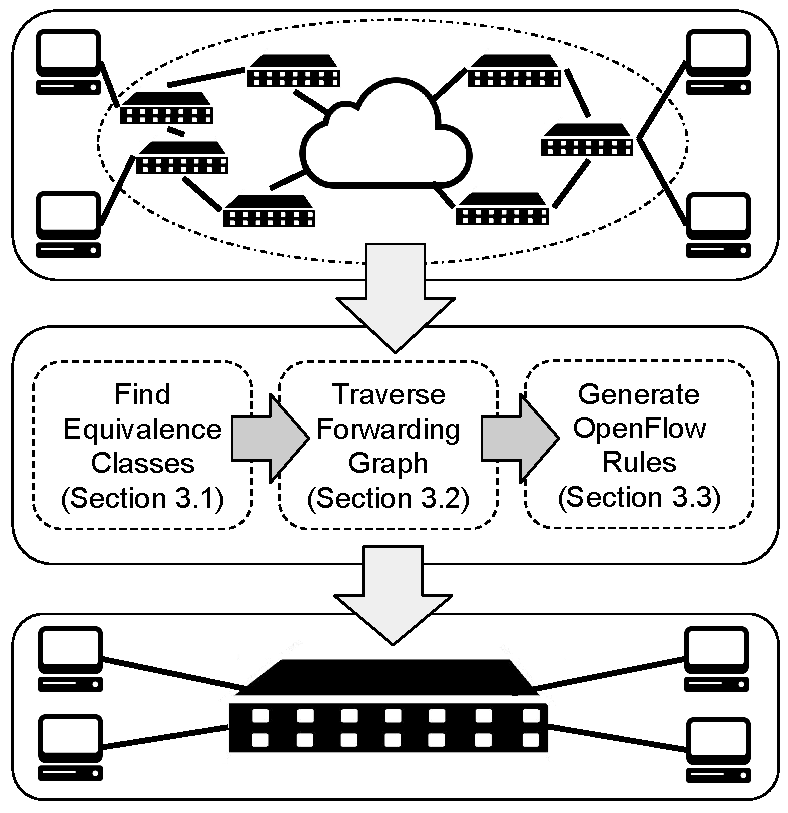
\includegraphics[scale=.6]{figures/BigSimOverview.pdf}
\caption{Overview of BigSim}
\label{Fig:BigSimOverview}
\end{figure}

We have sketched the process of how to replace a OpenFlow-switch-connected network
with a single OpenFlow switch in section~\ref{Sec:MotivationalExample}.

In this section, we elaborate the details and relevant algorithms
in each procedure.

\subsection{Finding Minimal Set of ECs}
By aggregating and slicing forwarding rules in a SDN network to ECs,
one can obtain a compact representation of all the classes of network flows.
\begin{definition}
Equivalence Class (EC) is the set of packets that
experience identical forwarding action at \textbf{any} network device.
\end{definition}
Inspired by VeriFlow\cite{Veriflow}, we aggregate forwarding rules using a trie
compositing by several sub-tries, each representing one header field.
In the tree-topology network, for example, the trie is just a single sub-trie that
corresponds to the packet header (network-layer destination address)
part of the rule match field.


\subsubsection{Disjoint EC as Disjoint Intervals}
By traversing from root node to a leaf node, we can obtain one set of packets
that a rule matches.
All the leaves thus contains all the rules in the network.
However, these rules are not independent and may overlapping with each other.
In essential, each rule is an range of packet header values;
the set of rules are thus a list of ranges $R$ where $\forall r \in R$ can be
described by a pair of starting header value and ending header value.
Finding the set of disjoint ECs requires us to splitting $R$ to
a list of non-overlapping intervals.
Not algorithmic described in\cite{Veriflow},
we show this task can be accomplished in $O(N \times M\log M)$ time,
where $M=|R|$ is the number of intervals and $N$ is the total number of header bits,
as follows\cite{SplitDisjointInterval}.

First we unzip $R$ into an array $A$ of $2M$ values,
each flagged as either a start $S$ or an end $E$ of a range.
\footnote{Equal values with same flag are reduced to an single element.}
Before iterating $A$, we sort it, breaking the tie by putting $S$ point before $E$ point.
Then we maintain the difference $d$ between the number of $S$ points and the number of $E$ points
seen so far, while visit each point in sorted order:
\begin{itemize}
\item If current element $x$ is $S$ and $d > 0$,
        we end the previous interval with ending value $x - 1$.
        start a new interval with starting value $x$
        (line~\ref{Alg:LineEndStart1}-\ref{Alg:LineEndStart2}).
\item If current element $x$ is $E$, we end the previous interval with ending value $x$.
        (line~\ref{Alg:LineEndEnd}).
\item In either case, we update the potential new interval's start value \textit{prev}
        (line~\ref{Alg:LineNewPrev1} and \ref{Alg:LineNewPrev2}).
\end{itemize}

Updating forwarding rules in the network will result in the change of EC set.
By maintaining the rules in a trie, we can efficiently update ECs incrementally as follows.
Inserting new rule to the trie require us to do a depth-first-style trie traverse.
This process automatically narrows down the affected rules by ignore the branches
that is impossible to overlap with the newly inserted rule.
The result of the procedure is the set of the effected ranges.
We only need to run Algorithm~\ref{Alg:GenDisjointECs} to update ECs in the effected ranges.

\begin{algorithm}[h]
\DontPrintSemicolon
\KwData{$R = $ set of rules from the leaf-node of the trie}
\KwResult{$EC = $ set of equivalence classes as disjoint intervals}
$cnt \gets 0$\;
$S = $ \{start points of $\forall r \in R\}$, $E = $ \{end points of $\forall r \in R\}$\;
$A \gets Sort(S \bigcup E)$ in non-decreasing order\;
$EC \gets \emptyset$\;
\ForEach {$x \in A$} {
        \uIf {$x \in S$} {
                \If {$cnt \neq 0$} {\label{Alg:LineEndStart1} 
                        $EC \gets EC \text{ }\bigcup \text{} [prev, x-1]$\;
                }\label{Alg:LineEndStart2} 
                $prev \gets x$\;\label{Alg:LineNewPrev1}
                $cnt \gets cnt + 1$\;
        }
        \Else ($x \in E$) {
                $EC \gets EC \text{ } \bigcup \text{ } [prev, x]$\;\label{Alg:LineEndEnd}
                $prev \gets x + 1$\;\label{Alg:LineNewPrev2}
                $cnt \gets cnt - 1$\;
        }
}
\caption{Generate Disjoint ECs\label{Alg:GenDisjointECs}}
\end{algorithm}

\subsubsection{Minimal EC Set}
The resulting disjoint EC set $ECS$ obtained from Algorithm~\ref{Alg:GenDisjointECs} are unfortunately not the optimal one with minimum size.
Many ECs can be merged together.
For example, EC1 and EC3 in section~\ref{Sec:MotivationalExample} can be seen as one EC.
By the definition of EC, since $\forall d$ takes identical forwarding action for any one of
the mergeable ECs, we have:
\begin{lemma}
A set of mergeable disjoint ECs has the same forwarding graph.
\label{Lemma:MergeFG}
\end{lemma}
Thus, operating on the minimal EC set can reduce running time in the later phase of
generating forwarding graph as well as populating final OpenFlow rules.
Here we provide a solution with its proof.
Our solution builds on the following Lemma.
\begin{lemma}
A pair of disjoint ECs in $ECS$ is mergeable if they intersect with
the same set of rules in the network.
\label{Lemma:MergeEC}
\end{lemma}
The proof of Lemma~\ref{Lemma:MergeEC} is as follows.
Let $\alpha$ and $\beta$ be two ECs that intersect with the same set of rules $\Delta$.
At $\forall$ network device $d$, let $\delta \in \Delta$ be the rule on $d$ with
highest priority.
If no such $\delta$ exist, packets from both $\alpha$ and $\beta$ are dropped on $d$.
Otherwise, device $d$ will forward packets from both $\alpha$ and $\beta$ according to the same
rule $\delta$.
By the definition of EC, packets in $\alpha$ and $\beta$ can be merged as one single EC
since at any network switch they have identical forwarding action.

Finding the list of rules $\Delta[\alpha]$ that intersects with EC $\alpha$ can be done
efficiently with two data structure,
each taking care one of the two cases\cite{FindIntersectionWiki}:
\begin{itemize}
\item Rule $\delta$ intersects $\alpha$ with its start and/or end point in $\alpha$.
        We can reuse the sorted array $A$ in Algorithm~\ref{Alg:GenDisjointECs}.
        Here we assume we augmented each value in $A$ with a pointer that points to
        the rule it belongs to.
        By doing binary search, we can find the minimum and maximum value in $A$ that
        are in the range of $\alpha$.
        All intervals that intersect with $\alpha$ must be contained between
        the minima and maxima.
        We can then do linear search in this reduced list of ranges $A'$,
        check one by one if the interval that value $a\in A'$ belongs to
        intersects with $\alpha$.
        The total time complexity for both linear and binary search is thus $O(\log M + K)$,
        assuming $K=|\Delta|$ is the number of reported intervals.
\item Rule $\delta$ covers $\alpha$ entirely. We can build
        a central interval tree\cite{ComputationalGeometryBook} using all available ranges.
        We pick a random value $x \in \alpha$ and query the central interval tree for
        all ranges that intersect with $x$, which can be done in $O(\log M + K)$ time,
        at the cost of $O(M log M)$ time for building the central interval tree. 
\end{itemize}

For each EC $\alpha$ we have found the list of intervals $\Delta[\alpha]$
that intersects with it with both interval tree and ordered list of boundary values.
By mapping each rule to an unique binary ID of length $\log_2 M$,
we can encode $\Delta[\alpha]$ to a string $C_\alpha$ of at most length $M\log_2 M$, putting
small binary IDs before large ones.
Then we use a hash table $H$ to group mergeable ECs by hashing each EC $x$ to $C_x$.
The minimal size of ECs is the number of unique keys in $H$.
In the later text, when we say ``iterate through all (disjoint) ECs" or "for each EC" etc,
we are actually visiting the first ECs in each set $H[key]$, $\forall key \in H$.


\subsection{Generating Forwarding Graphs}
In the second stage, we compute forwarding graphs for each EC and
compress them in order to be used in the next stage.
Forwarding graph not only concatenates the forwarding actions of each EC,
but also visualizes the flow the EC.
For a fixed EC $x$, we connect the network devices that have rules for $x$
with directed edges that point to the next hop,
which is available in the action field of the rule.
Since our goal is to compress the network logic, we are more interested in the sources
and sinks of the directed graph.

We define \textit{edge switches} as these switches whose port will be remapped to the port on
the resulting big switch;
in contrast, \textit{internal switches} are abstracted away in the final big switch.
Forwarding graphs are generated by starting from each \textbf{edge switch} and traversing
in the depth-first-search style by following the action of the highest-priority rule
covering EC $x$.
Source node $src$ and its out-going edge represent an edge switch $sw$ that
forwards EC $x$ \textbf{coming from} port $p$; it can be described by $(sw, p)$ pair.
Sink node $snk$ represent the end of the forwarding $sw$,
which is also denoted by $(sw, p)$, where $p$ is either the port number
specified by the action field or \texttt{NULL} if there is no rule for $x$ on $sw$.
%We denote the set of source nodes as $SRC(x)$, the set of sink nodes as $SNK(x)$.
Notice that (1) source nodes in $FG(x)$ can only be edge switch,
while it is possible that sink nodes are inner switches;
(2) the inner graph between sink and source may contain both edge and internal switches.

We depict the generalized forwarding graph $FG(x)$ for EC $x$
in Figure~\ref{Fig:SummaryForwardingGraph}.
We add a super-source node $SRC^x$and a super-sink node $SNK^x$, both represent the EC $x$.
For convenience in discussion, we distinguish two kinds of port on \textbf{edge switch}es:
\textit{end port} connects to endpoints or the outside of the network we are abstracting, while
\textit{inner port} connects to another network device inside the network we are abstracting.
We add an edge from $SRC^x$ to a source node(edge switch) $src$ if
\begin{enumerate}
\item the edge switch has a forwarding rule $r$ that covers EC $x$;
\item the $IN\_PORT$ field of $r$ corresponds to an \textbf{end port} of the edge switch
\end{enumerate}
otherwise, we don't need to initiate traverse at all
(see line~\ref{Alg:LineStartDFS1} to \ref{Alg:LineStartDFS2}
in Algorithm~\ref{Alg:GenForwardingGraph}).
Correspondingly, we add an edge from a sink node $snk$ to super sink $SNK^x$
if both conditions are satisfied:
\begin{enumerate}
\item the sink node is representing an edge switch in the network;
\item the $OUT\_PORT$ field determined by the rule's action on the edge switch is \textbf{end port}
\end{enumerate}

Using the depth-first-search algorithm shown in Algorithm~\ref{Alg:GenForwardingGraph},
we can discover three kinds of ``path" in $FG(x)$ that related to rule generation on
the big virtual switch:
\begin{itemize}
\item \textbf{Forwarding Path}(line~\ref{Alg:LineForwardPath1}-\ref{Alg:LineForwardPath2}).
        The path, starting from super source,
        leads to super sink node through a end port on another edge switch to host.
        This is a normal forwarding path for packets $\in$ EC $x$.
\item \textbf{Dropped in the Middle}(line~\ref{Alg:LineDropPath1}-\ref{Alg:LineDropPath2}).
        The path ends inside the graph, unable to arrive
        at the super sink node. This path tell us that packets
        defined by EC $x$ are dropped, at least partially,
        in some intermediate switch in the network.
\item \textbf{Forwarding Loop}(line~\ref{Alg:LineLoopPath}).
        There is a directed cycle in the graph, which can be
        detected during the depth-first-search traverse.
        This behavior can be emulated in the semantic of \textbf{performance equivalence},
        but not by \textbf{logical equivalence} studied in this paper.        
        For example, we can emulate a forwarding loop in the network by
        (1) recording the volume of the looping packets;
        (2) increasing the delay of other packets on the basis of the amount of looping packets
        (3) adding a rule so that looping packets are dropped by big switch;
\end{itemize}

\begin{algorithm}[h]
\DontPrintSemicolon
\KwIn{$nodes = $ Switches that have rule for $x$ \newline
        Topology of the network $topo$}
\KwResult{Forwarding graph $FG(x)$ for EC $x$}
\SetKwProg{Fn}{Function}{}{\KwRet}
\SetKwFunction{Traverse}{traverse}
\SetKwFunction{GenRule}{generate\_rules}
\Fn{\Traverse{$curr$, $src$, $snk$}} {
        \uIf {$curr$ \upshape is \textbf{NOT} visited} {
                $r \gets$ \textbf{highest-priority} rule on $curr$ that covers $x$\;
                \If {r \upshape is NULL or $r.action$ is DROP} {\label{Alg:LineDropPath1}
                        $snk \gets$ ($curr$, NULL)\;
                        \GenRule{$x, src, snk$}\;
                        \KwRet\;
                }\label{Alg:LineDropPath2}
                $next \gets topo[curr][r.action.outport]$\;
                \If {next $\not\in$ nodes} {\label{Alg:LineForwardPath1}
                        $snk \gets$ ($curr$, $r.action.outport$)\;
                        \GenRule{$x, curr, src, snk$}\;
                        \KwRet\;
                }\label{Alg:LineForwardPath2}
                mark $curr$ as visited\;
                \Traverse{$next, src, snk$}\;
        }
        \Else {
                report forwarding loop\;\label{Alg:LineLoopPath}
        }
}\;
\ForEach{$n \in$ \upshape neighbors of $SRC^x$} {\label{Alg:LineStartDFS1}
        \If {\upshape $n$ is \textbf{NOT} visited} {
                $inport \gets$ inport number from $SRC^x$ to $n$\;
                \Traverse{$n$, $src=$\upshape($n$, $inport$), $snk=$NULL}\;
        }
}\label{Alg:LineStartDFS2}
\caption{Generate Forwarding Graph for EC $x$\label{Alg:GenForwardingGraph}}
\end{algorithm}


\subsection{Populating Flow Table on Big Switch}

Depending on the kind of path, we can easily generate OpenFlow rules on the abstracted
big switch at the end of forwarding graph traversal by calling \texttt{generate\_rules},
which is described in Algorithm~\ref{Alg:GenAllRules}.
We maintain a hash table $PortMap$ to map end ports on edge switches to the big virtual switch.
This table is configured as rule generation using $global\_port$ variable.
Algorithm~\ref{Alg:GenAllRules} fills the mandatory fields in an OpenFlow rule:
\begin{itemize}
\item The $MATCH$ field is given by the EC $x$ itself, e.g. the range of matching packets header
        (line \ref{Alg:LineMatch})
\item The $IN\_PORT$ field is the mapped port number of $src.port$ (line~\ref{Alg:LineInport})
\item Depending on the $dst$'s port, we generate either a drop action
        (line~\ref{Alg:LineGenDropRule})
        or a forward action with appropriate mapped port number of $dst.port$ 
        (line~\ref{Alg:LineGenForwardRule1}-\ref{Alg:LineGenForwardRule2})
\end{itemize}



\begin{algorithm}[h]
\DontPrintSemicolon
\KwData{$PortMap$ maps $port$ on $sw$ $\rightarrow port$ on big switch\newline
        $global\_port$ assigned to unseen port number}
\KwResult{New rule $r$ to install in $BS$}
Assume $global\_port$ is globally initialized to 0\;
\SetKwProg{Fn}{Function}{}{\KwRet}
\SetKwFunction{GenRule}{generate\_rules}
\Fn{\GenRule{$x, src, dst$}} {
        $r.match \gets x$\;\label{Alg:LineMatch}
        \If {src.port $\not\in$ PortMap[src.sw]} {
                $PortMap[src.sw][src.port] \gets global\_port++$\;
        }
        $r.inport = PortMap[src.sw][src.port]$\;\label{Alg:LineInport}
        \uIf {dst.port \upshape is NULL} {
                $r.action \gets $ drop\_action\;\label{Alg:LineGenDropRule}
        }
        \Else {
                \If {dst.port $\not\in$ PortMap[dst.sw]} {\label{Alg:LineGenForwardRule1}
                        $PortMap[dst.sw][dst.port] \gets global\_port++$\;
                }
                $r.action \gets $ forward\_action\;
                $r.action.outport \gets PortMap[dst.sw][dst.port]$\;\label{Alg:LineGenForwardRule2}
                
        }
}
\caption{Generate Rule for EC $x$ on Big Switch\label{Alg:GenAllRules}}
\end{algorithm}




\section{Evaluation}

\begin{figure*}[h]
        \centering
        \subfloat[$\mathcal{R}_1$, packets received per host in $net_1(d=2, f=3)$] {
                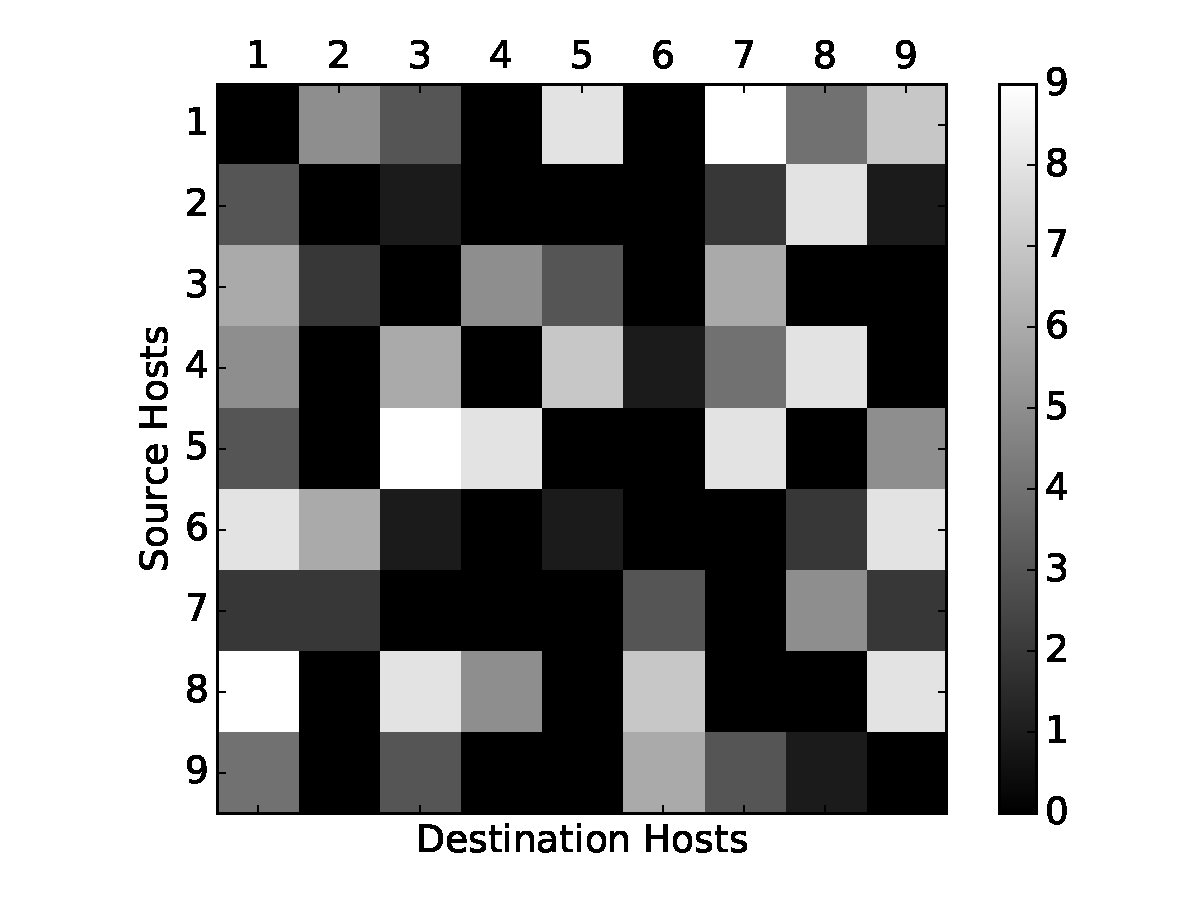
\includegraphics[scale=.42]{figures/ping_mat_2_3.pdf}
                \label{Fig:PingMatrix1}
        }
        \subfloat[$\mathcal{R}_2$, Packets received in $net_2(d=2, f=3)$] {
                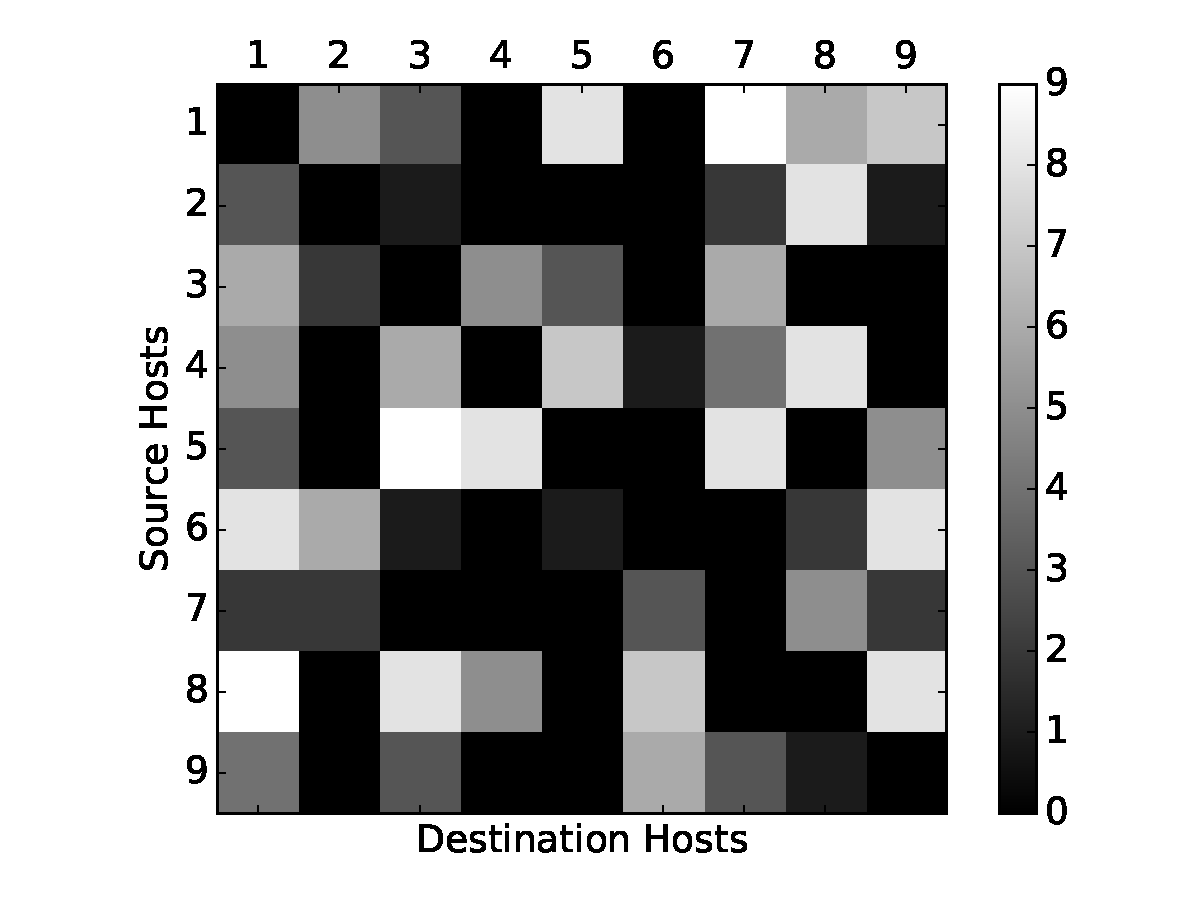
\includegraphics[scale=.42]{figures/bs_ping_mat_2_3.pdf}
                \label{Fig:PingMatrix2}
        }
        \\
        \subfloat[$\mathcal{R}_1$, Packets received in $net_1(d=4, f=3)$] {
                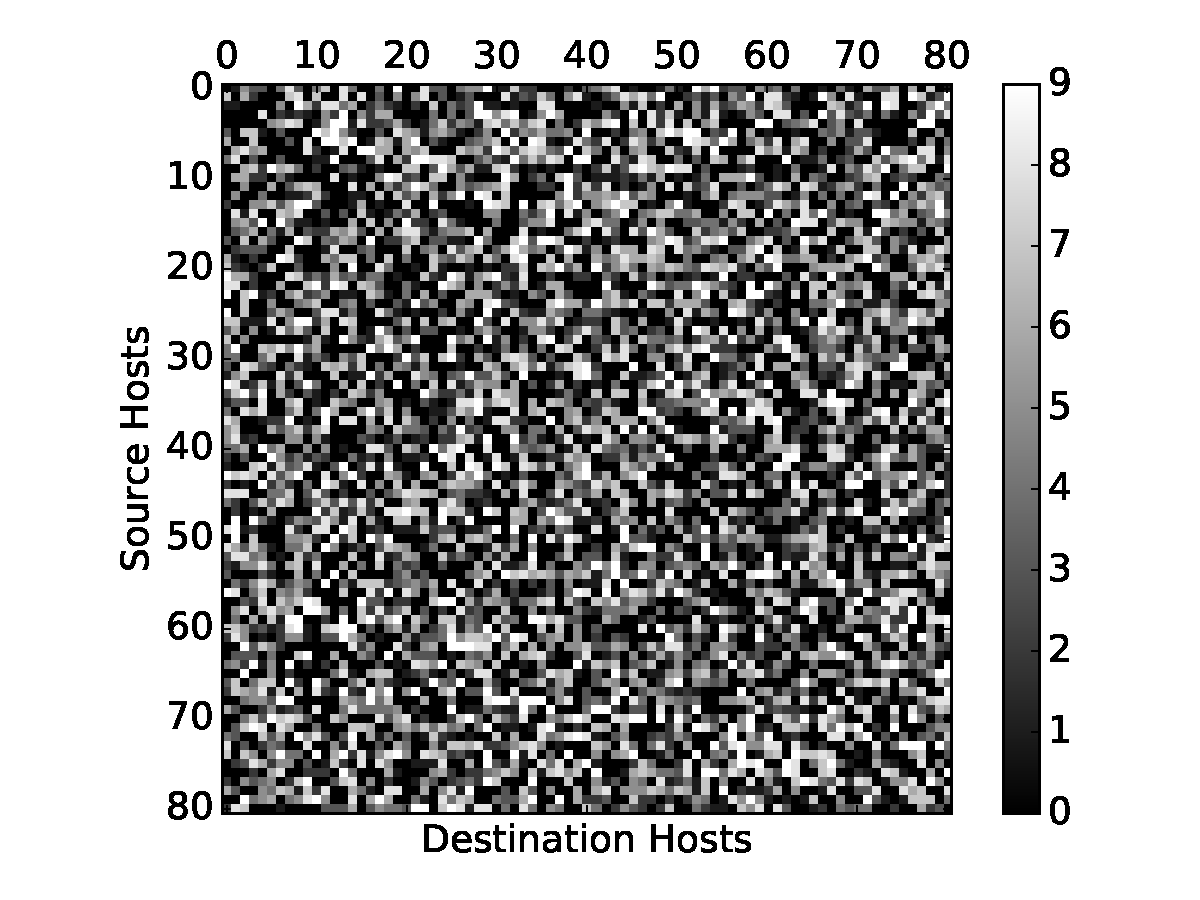
\includegraphics[scale=.42]{figures/ping_mat_4_3.pdf}
                \label{Fig:PingMatrix3}
        }
        \subfloat[$\mathcal{R}_2$, Packets received in $net_2(d=4, f=3)$] {
                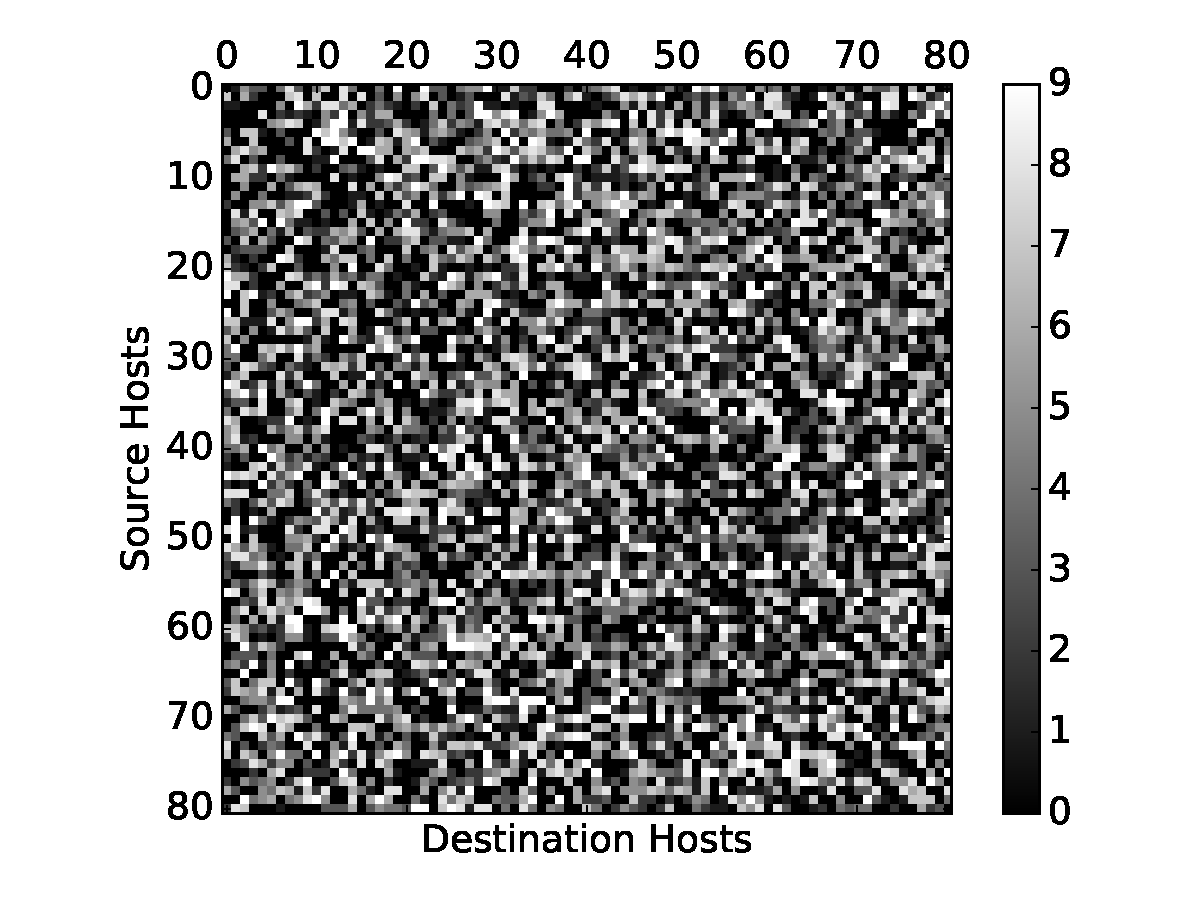
\includegraphics[scale=.42]{figures/bs_ping_mat_4_3.pdf}
                \label{Fig:PingMatrix4}
        }
        \caption{
        Matrix $\mathcal{R}$ represents the number of packets received at each host.
        $net_1$ is the original SDN network with a tree topology ($d$, $f$),
        where $d$ is depth and $f$ is fanout.
        $net_2$ is the corresponding one-big-switch-based network.
        The gradient legend visualizes the number of received packets.
        $\mathcal{R}_1$ and $\mathcal{R}_2$ are identical,
        which indicate that our model abstraction technique preserves the network forwarding logic.}
        \label{Fig:ComparePingMatrix}
\end{figure*}

\begin{figure}[h]
\centering
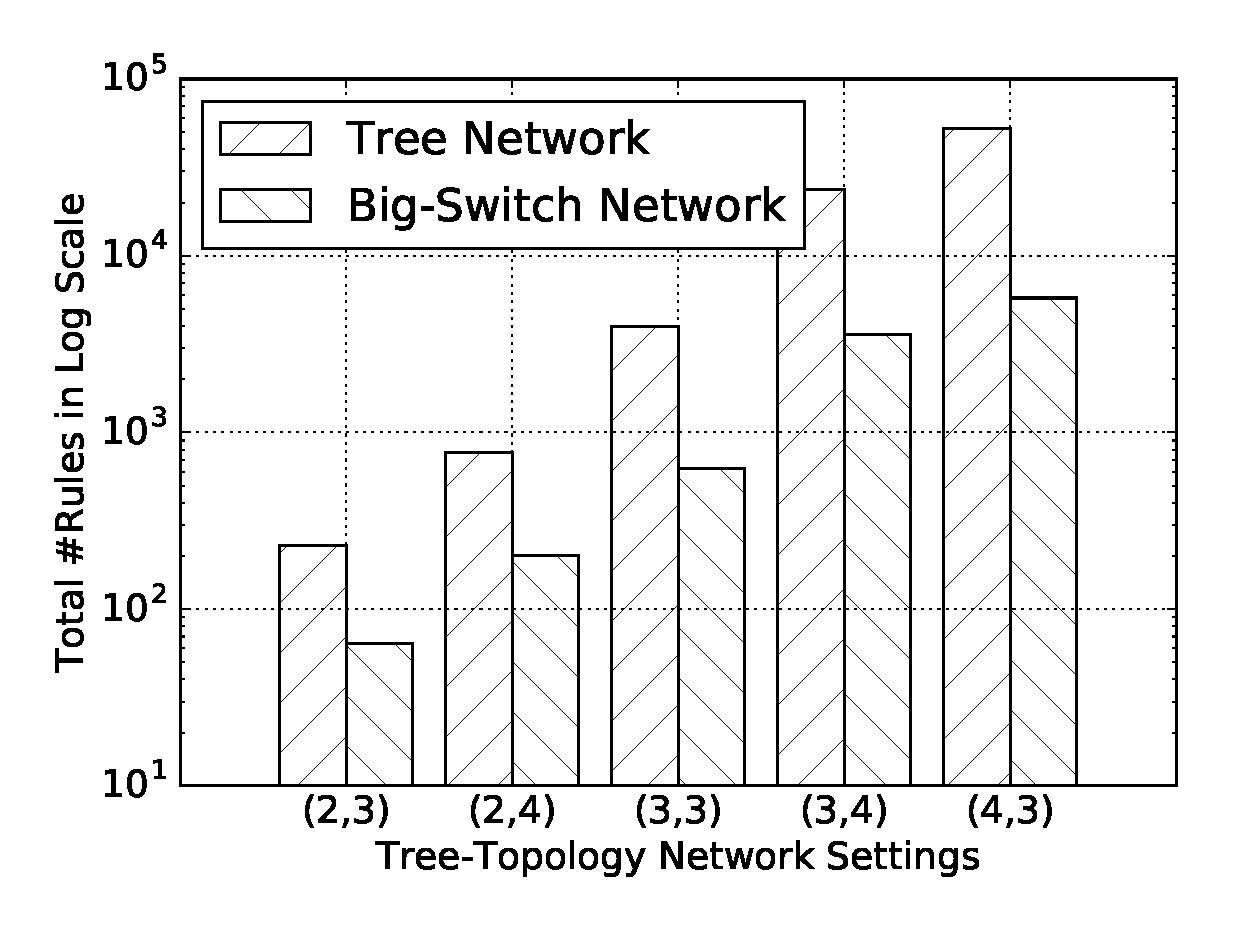
\includegraphics[scale=.42]{figures/comp_num_rules.eps}
\caption{Number of rules needed to preserve the network forwarding logic.
        The number of rules on the big switch is about 72\% to 89\% less than
        the number of rules in the original tree-topology network.
        The x-axis label ($d$, $f$) represents the depth and fanout parameters
        in a tree topology network.}
\label{Fig:CompareNumRules}
\end{figure}


\begin{figure}[h]
\centering
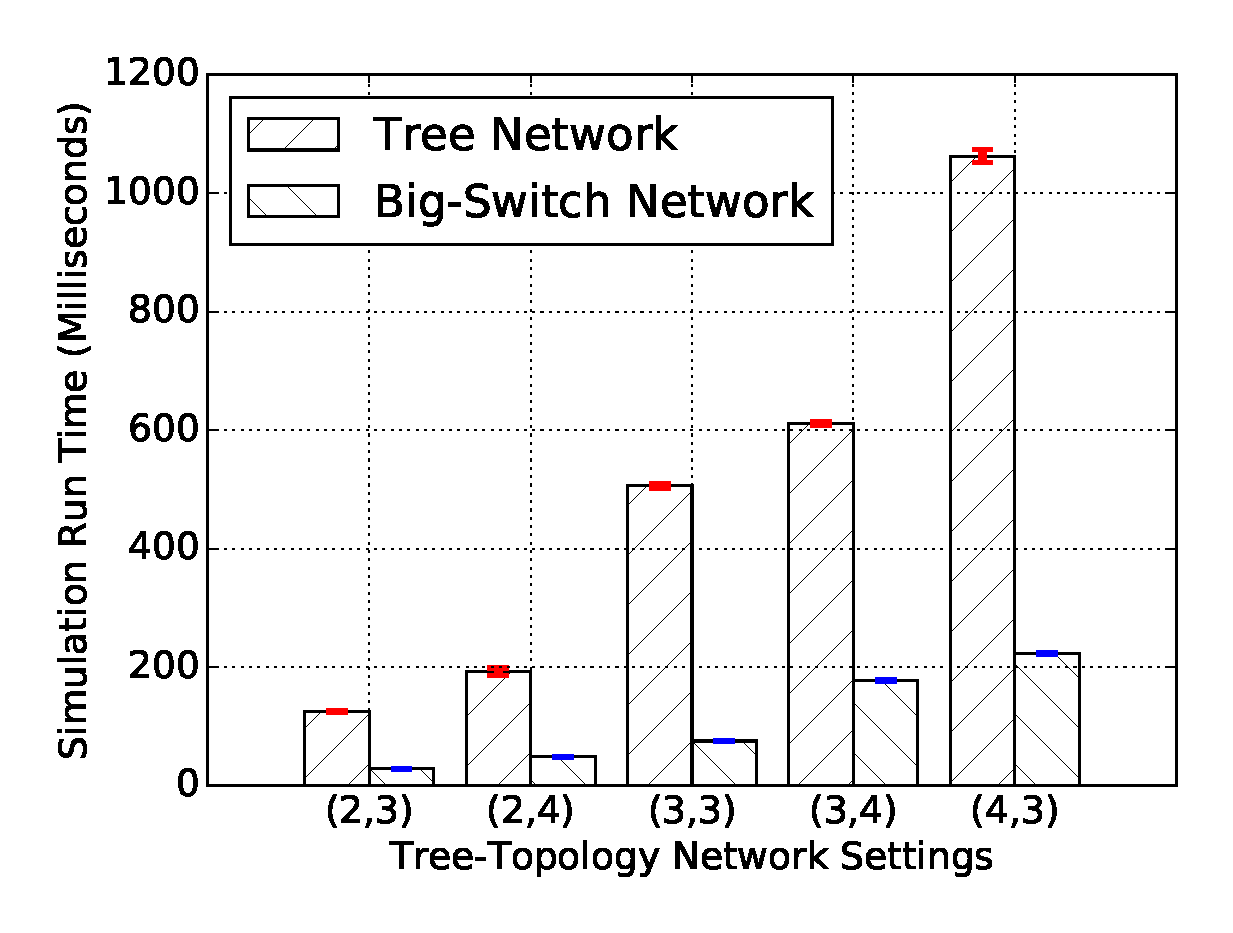
\includegraphics[scale=.42]{figures/comp_sim_time.eps}
\caption{Comparison of simulation execution time.
        The big-switch-based network model saves about 75\% to 85\% running time
        as compared to simulating the corresponding SDN-based network.
        The x-axis label ($d$, $f$) represents the depth and fanout parameters in a tree topology network.}
\label{Fig:CompareSimulationTime}
\end{figure}

\begin{figure}[h]
\centering
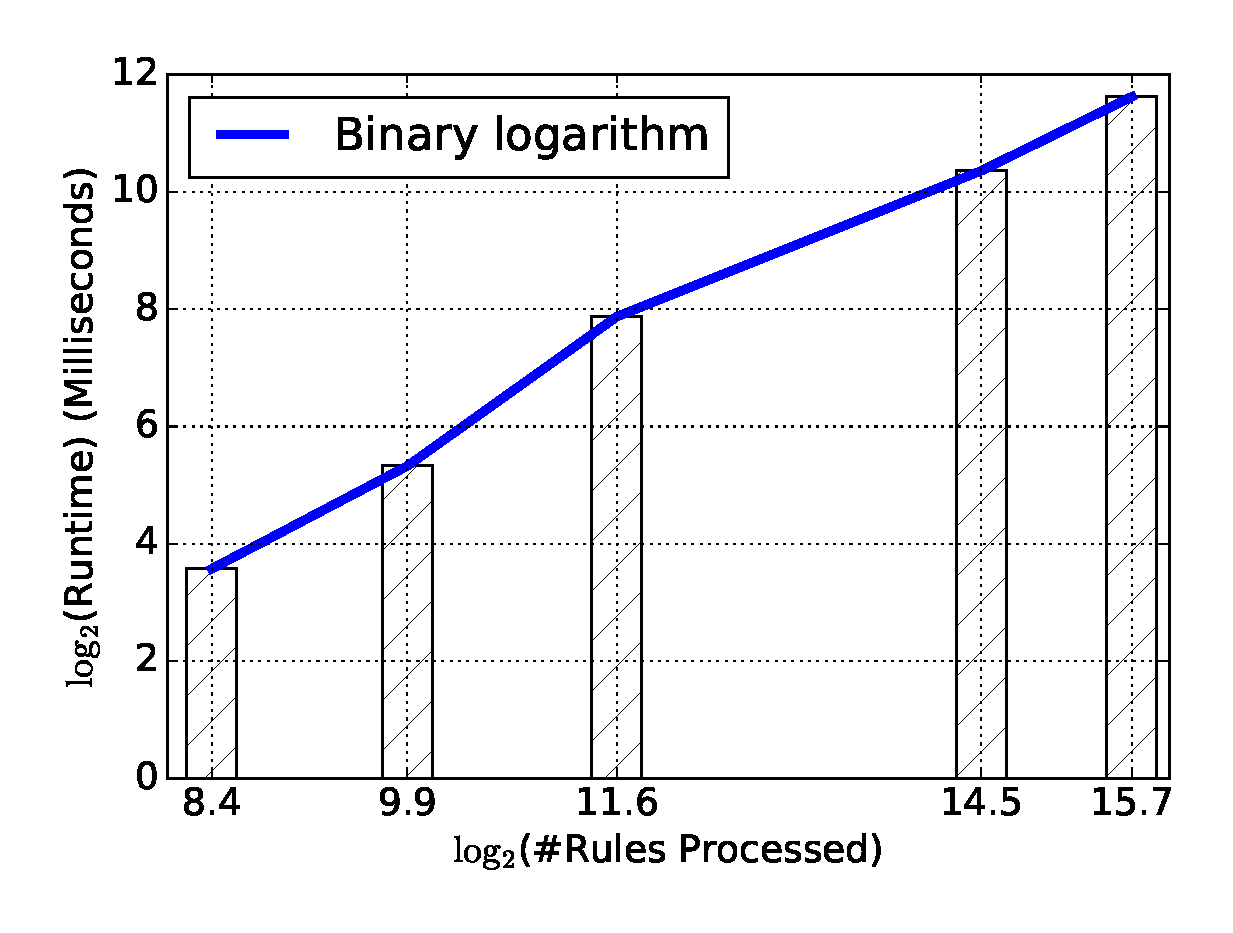
\includegraphics[scale=.32]{figures/bs_overhead.eps}
\caption{Execution time to transform an SDN-based network to a big-switch-based network.}
\label{Fig:BSOverhead}
\end{figure}

\subsection{Network Forwarding Logic Equivalence}
\label{SubSec:PreserveForwardingLogic}


We perform experimental evaluation of our network model abstraction technique
that transforms an SDN-based network to one big switch.
The evaluation results show that our approach significantly saves simulation/emulation resources
(e.g., number of forwarding rules) and simulation execution time,
while still preserving the forwarding behavior of the original network.

Our experiments simulate and emulate networks of type tree topology.
The tree network is described by two topological parameters: depth $d$ and fanout $f$.
Such network $tree(d, f)$ can connect $f^d$ hosts with $\frac{f^d - 1}{f-1}$ switches in total.
%Though not known as a scalable network architecture (a good scalable alternative will be fat-tree topology), it is good for demonstration purpose since the tree topology is well-structured and
All end-hosts in a tree network are fully-connected with at most $2d$ hops.


We first demonstrate that the forwarding logic of the original software-defined network is exactly preserved by the abstracted big switch model.
%One can find the shortest path between a pair of hosts $(s, d)$ with a layer-two learning switch controller application. Traversing the tree up and down in breadth-first-search style, learning switch application can automatically install OpenFlow rules on each hop once we initiate \texttt{ping} between the given pair of host. More specifically,
We created a tree-topology network $net_1$ in Mininet\cite{Mininet}, and connected all the switches to an SDN controller running a layer-two learning switch application \cite{Pox}. %We generated the network forwarding rules by establishing communication paths between random selected host pairs.
%For any network host $s$, we randomly generate a list of distinct hosts $dsts$, and let $s$ \texttt{ping} each host $dst \in dsts$.
After performing the \texttt{ping} tests between randomly selected pairs of end-hosts, the controller application generated all the network forwarding rules and installed them on the switches.
We then took a snapshot of the network, including (1) the host-to-switch and switch-to-switch connections, and (2) the rules on all the switches using the \texttt{ovs-ofctl dump-flows} command. The snapshot was used to generate the rules for the big switch model as well as the port mapping according to the algorithms presented in Section~\ref{Sec:Design}.

We then created another emulated network $net_2$ in Mininet, consisting of one OpenFlow switch and the same number of hosts as $net_1$.
The switch was connected to $f^d$ hosts with the port numbers derived from both the $PortMap$ (Algorithm~\ref{Alg:GenAllRules}) and the link information ($net_1$'s topology).
The rules generated by Algorithm~\ref{Alg:GenAllRules} were installed on the switch using the \texttt{ovs-ofctl add-flow} command.

To validate that the big-switch-network preserved the network forwarding logic of the original network,
we recorded the connectivity between \emph{every} host pair in both $net_1$ and $net_2$,
and compared the results.
Specially, the original network $net_1$ is a tree network with $f^d$ hosts,
where $d$ is the depth and $f$ is the fanout of a tree network.
Each host sent a number of \texttt{ping} packets to every other host in $net_1$,
and the amount of packet was randomly selected between 1 and 10.
We repeated the experiments in $net_2$ with the same traffic pattern.
The result was represented in a matrix $\mathcal{R}$,
where $\mathcal{R}[i][j]$ denotes the numbers of successfully received \texttt{ping}
packets from host $i$ to host j, where $i \neq j$, and $i, j \in [1, f^d]$.

%To prevent l2\_learning switch controller from installing new rules in $net_1$, we take down the pox controller in this stage.
%The result of this experiment is a matrix $\mathcal{R}_k$ where $\mathcal{R}[i][j]$ denote

We repeated the experiment for different combinations of $d$ and $f$, i.e., ($d, f$) $\in$
\{(2, 3), (2, 4), (3, 3), (3, 4), (4, 3)\}. For each network scenario,
we saved the experimental results in $\mathcal{R}_1$ and $\mathcal{R}_2$, and compared the two matrices using the \texttt{diff} command.
We found that $\mathcal{R}_1 = \mathcal{R}_2$ holds true for all five network scenarios.
We visualized $\mathcal{R}_1$ and $\mathcal{R}_2$ for the ($d=2, f=3$) and ($d=4, f=3$) cases
in Figure~\ref{Fig:ComparePingMatrix}.
We can see that the original SDN-based network and the abstracted one-big-switch-based
network have the identical network forwarding logic,
measured by the connectivity and the number of receiving packets for each connection.
%In Figure~\ref{Fig:PingMatrix1}-Figure~\ref{Fig:PingMatrix4},
Note that the brightness of the element in the matrix is proportional to $\mathcal{R}[i][j]$,
i.e., the number of successfully delivered packets from host $i$ to host $j$.
%It is easy to see that $\mathcal{R}_1$ and $\mathcal{R}_2$ are identical for all experiment settings.

\subsection{Performance Gain}

\textbf{Number of OpenFlow Rules.} We compare the total number of rules installed
on the switches in both $net_1$ and $net_2$ with the same experimental settings
in Section \ref{SubSec:PreserveForwardingLogic}.
The results are plotted in Figure~\ref{Fig:CompareNumRules} for networks with
various topological parameter settings.
%Note that y-axis is in log scale.
The number of rules needed to preserve the forwarding logic is significantly
less in the one-big-switch-based network as compared with the original SDN-based network
for all scenarios in the range of 71.93\% to 89.05\% reduction.
%approximately one degree of magnitude less than the number of rules existing in the original tree-topology network.
For example, in the case of a network with depth = 4, and fanout = 3, 52,660 rules
in the original network were reduced to 5,766 rules in the big-switch-based network.


\textbf{Simulation Time.}
Our approach significantly reduces network simulation model complexity in terms of
the number of switches and the number of rules.
A key benefit is to reduce the time to run simulation experiments.

We performed the same set of experiments on a network simulator, S3FNet \cite{S3F}.
We simulated two SDN-based networks: one models a tree-topology network $net_1(d, f)$,
and the other models the corresponding big-switch-based network $net_2$.
We set half of the hosts as TCP clients and the other half as TCP servers,
and conducted one-to-one communication among them.
We sent each traffic flow for 100 seconds in simulation time.
We repeated each experiment ten times and recorded the simulation execution time for both $net_1$ and $net_2$ in Figure~\ref{Fig:CompareSimulationTime} for comparison.
The error bars indicate the standard deviations of the running time
for all ten independent simulation runs.
We can see that simulating the big-switch-based network is 3.42 to 6.68 times
faster than simulating the original SDN-based network.


\subsection{Model Abstraction Execution Time}

We discussed the asymptotic time complexity of our model abstraction technique in 
Section~\ref{Sec:Design}.
We now evaluate the execution time for transforming an SDN-based network to a big-switch-based network.
We recorded the running time for converting various tree networks,
i.e., ($d, f$) $\in$ \{(2, 3), (2, 4), (3, 3), (3, 4), (4, 3)\} in Figure~\ref{Fig:BSOverhead}.
We can see that the model abstraction process is lightweight.
For example, it took about 40 milliseconds to abstract a small tree network ($d=4$, $f=2$);
for a medium-scale medium-scale tree network (depth 4 and fanout 3),
it took about 3.15 seconds to process 52,660 rules.
The fast model abstraction execution time is useful.
As the network state keeps evolving, it is essential to constantly update the abstracted big switch model to reflect the changes, preferably in an online fashion.
In fact, the three-step approach allows us to incrementally update the big switch model and requires far less execution time, i.e.,
we only need to update a small set of rules that are different in the new network snapshot.

%Since the network is constantly being reconfigured to han- dle the changing requirements and dynamic events, the trans- formed �big switch� also need to change correspondingly to enable online simulation/emulation.
%The overhead of our approach is that we need to process the existing rules in the original network, map the original topology to a single-switch topology, and generate new rules. In practice this process can be done offline once, as we did in the experiments above, and the newly generated rule can be installed in multiple runs thereafter.
%Since the scale of the experiment increases exponentially, we put both x-axis($nr$) and y-axis ($rt$) in binary log scale ($\log_2$).
%It is clear that our approach scale linearly as the input size increases in the scenario of this tree-topology network.



\section{Conclusion and Future Works}

In this paper we showed that a SDN network can be reduced to a simple OpenFlow switch
without the loss of the forwarding logic defined by all the rules in the network.
We proposed a three-step solution to this abstraction problem.
First we slice all the possible packets in the network into equivalence classes.
Then we build forwarding graphs for each equivalence class.
By traversing forwarding graphs, we can generate new rules to be installed
on the big switch.
Experiment demonstrates that the big switch abstracted by our approach correctly models
the end-to-end forwarding behavior of the SDN network with tolerable computational overhead.
Simulation running time can be reduced using our big-switch model.
In the future, we plan to solve the problem of how to preserve the end-to-end latency
equivalence.



%ACKNOWLEDGMENTS are optional
\section{Acknowledgments}
The author would like to thank the authors of ~\cite{Veriflow} share the Veriflow codebase
for research purpose .
This paper is partly sponsored by the Maryland Procurement Office under Contract No. H98230-14-C-0141,
and the Air Force Office of Scientific Research (AFOSR) under grant FA9550-15-1-0190.
Any opinions, findings and conclusions or recommendations expressed in this material are
those of the author(s) and do not necessarily reflect the views of
the Maryland Procurement Office and AFOSR.


%\end{document}  % This is where a 'short' article might terminate

%
% The following two commands are all you need in the
% initial runs of your .tex file to
% produce the bibliography for the citations in your paper.
\bibliographystyle{abbrv}
\bibliography{sigproc}  % sigproc.bib is the name of the Bibliography in this case
% You must have a proper ".bib" file
%  and remember to run:
% latex bibtex latex latex
% to resolve all references
%
% ACM needs 'a single self-contained file'!
%

%\nocite{*}
%\balancecolumns % GM June 2007
% That's all folks!
\end{document}
